\documentclass{Academic}

\usepackage{booktabs}
\usepackage{makecell}
\usepackage{graphicx}

\begin{document}
%Easy customisation of title page
%TC:ignore
\myabstract{\small
\noindent\textbf{Resumen}
%Abstract below

La enfermedad renal crónica (ERC) es una pérdida progresiva de la función renal que afectó a más de 800 millones de personas en 2017, 
con frecuencia subdiagnosticada por presentar síntomas en etapas avanzadas. Su detección temprana podría reducir significativamente su 
carga clínica y económica. El siguiente estudio empleó un enfoque cuantitativo no experimental basado en redes bayesianas gaussianas (GBN) 
para modelar las relaciones de dependencia probabilística entre biomarcadores clínicos asociados a la ERC, utilizando la base de datos 
ckd.csv. Se construyeron tres grafos acíclicos dirigidos (DAGs) con distintos subconjuntos de variables, definidos con apoyo de estudiantes 
y profesores de medicina, ajustados con bn.fit() en R mediante el paquete bnlearn y evaluados utilizando los criterios BIC y AIC. La DAG 2 
presentó el mejor desempeño global y fue seleccionada para realizar las consultas probabilísticas propuestas por especialistas. Los 
resultados mostraron probabilidades de 62.77 % de creatinina sérica elevada dado un nivel alto de sodio, 62.84 % al considerar 
simultáneamente sodio y potasio elevados, 43.13 % de hiperpotasemia ante creatinina y urea elevadas, 80.96 % de hemoglobina menor a 12 g/dL 
ante una creatinina de 3.0 mg/dL y un conteo de eritrocitos de 3.5 millones/\(\mu\)L, y 100 % de creatinina elevada ante presión arterial 
superior a 140 dentro del modelo ajustado. Asimismo, el modelo no paramétrico mejoró los valores de BIC y AIC de la DAG 2 respecto al modelo 
lineal, aunque las consultas probabilísticas se realizaron sobre este último. Finalmente, se identificó como limitación la imposibilidad de 
incorporar directamente variables categóricas, como el diagnóstico de ERC, en una red exclusivamente gaussiana, proponiéndose como extensión 
futura el uso de redes bayesianas gaussianas condicionales o redes discretas.
}
\renewcommand{\myTitle}{Uso de Redes Bayesianas Gaussianas para comprender 
el efecto de biomarcadores en la Enfermedad renal crónica: Un análisis probabilístico}
\renewcommand{\MyAuthors}{%
    Jessica Milagros Cordero Rivera$^{1}$ \quad
    Diego Rodrigo González Ramírez$^{1}$\\[0.2em]
    Jose Ángel Lechuga Carrasco$^{1}$ \quad
    Julio Lizárraga Beltrán$^{1}$
}

\renewcommand{\MyAffiliations}{%
    $^{1}$Escuela de Ingeniería y Ciencias
}

\renewcommand{\AuthorIDs}{%
    A01647083 \;|\; A01647198 \;|\; A00228198 \;|\; A01743628
}

\renewcommand{\ShortAuthors}{Cordero Rivera et al.}

\renewcommand{\Keywords}{enfermedad crónica renal, red bayesiana, red bayesiana gaussiana, asistencia médica, análisis probabilístico}
\maketitle
%\vspace{-1.9em}\noindent\rule{\textwidth}{1pt} %add this line if not using abstract
\onehalfspacing
%TC:endignore

\section{Introducción}


La enfermedad renal crónica (ERC) es la pérdida progresiva de la función de los riñones, 
afectando su función de eliminar residuos y exceso de agua del cuerpo. Al encontrarse
en una etapa tardía del ERC el paciente puede experimentar síntomas como, entre otros:

\begin{itemize}
  \item Piel anormalmente oscura o clara
  \item Dolor de huesos
  \item Problemas para concentrarse o pensar
  \item Fasciculaciones musculares o calambres
  \item Susceptibilidad a hematomas
  \item Sed excesiva
  \item Hinchazón en las manos y en los pies
\end{itemize}

A muchas personas no se les diagnostica la ERC sino hasta que han perdido 
gran parte de su función renal.\cite{definicion}. 
En 2017 la ERC afectó a más de 800 millones de personas y su tasa de mortalidad ha 
estado en aumento en este siglo. Además, debido a otras enfermedades cómo la diabetes mellitus 
y la obesidad, el riesgo de padecer ERC aumenta aún más y con ello, sus complicaciones \cite{Csaba}.

Es evidentemente claro que la identificación y diagnóstico de la ERC beneficiaría; para unas, 
La calidad de vida de millones de personas que podrían desarrollar esta enfermedad en un 
futuro; y para otras, evitar fallecer por esta enfermedad o complicaciones derivadas de ella. 
Los estudios epidemiológicos han concientizado sobre el problema de la ERC no 
diagnosticada y sugieren que su detección y tratamiento tempranos reducirán
la carga mundial que suponen los pacientes que necesitan diálisis \cite{Taal}.

Sin embargo, la prevención y diagnóstico temprano de la ERC no es una tarea sencilla, 
esto se debe principalmente a que hay una gran cantidad de factores que afectan al 
desarrollo de esta enfermedad: La dieta, consumo de drogas, predisposición genética, 
y otras enfermedades son posibles factores a considerar para la detección temprana de la 
ERC. Esta idea fue explorada por Taal et al. Proponen que los factores de riesgo de progresión de la ERC se
incorporen a un sistema de puntuación multivariable que permita
predecir el riesgo futuro de un individuo de padecer insuficiencia renal terminal. Esto permitiría
realizar pruebas específicas de la ERC en la población e identificar a
los pacientes con alto riesgo de progresión de la ERC para aplicarles una
intervención más intensiva. \cite{Taal}.

El uso de biomarcadores para la predicción del desarrollo de la ERC ha sido explorada
de manera muy efectiva por Navdeep et al. Dónde se realizaron diversos modelos predictivos con el 
objetivo de poder validar los modelos que predigan la progresión de la ERC. El modelo 
más preciso incluía la edad, el sexo, la Tasa de Filtración Glomerular estimada, la albuminuria, 
el calcio sérico, el fosfato sérico, el bicarbonato sérico y la albúmina sérica. \cite{Navdeep}.
Esto nos muestra la importancia de los biomarcadores para la predicción de la ERC.

Si bien estos enfoques muestran ser bastante efectivos, nuestro trabajo será enfocado hacia el análisis 
de los biomarcadores de una persona a través de una red bayesiana gaussiana (GBN).Las GBN son modelos 
probabilísticos que permiten mostrar las relaciones de causalidad entre distintas
variables numéricas con distribución normal utilizando un DAG. Las redes bayesianas resultan útiles para modelar 
problemas médicos complejos que requieren razonamiento en condiciones de incertidumbre. El gran interés 
que se muestra este tema queda reflejado en la abundante bibliografía que propone redes de Bayes para el 
ámbito médico y en el esfuerzo que se está dedicando a nivel mundial al desarrollo de estas redes para apoyar 
la toma de decisiones clínicas \cite{Kyrimi}. 

En este trabajo se utiliza la base de datos \texttt{ckd.csv}, una base de datos que contiene 400 registros sobre 
diferentes marcadores para una muestra de pacientes con y sin ERC. Con la informacion numérica disponible
se construyeron tres GBN. El modelo busca analizar las relaciones probabilísticas entre distintos 
biomarcadores de los pacientes de la base de datos. Posterior a ello se realizaron seis consultas probabilísticas 
orientadas a estudiar cómo el nivel de ciertos biomarcadores afectan a otros, y cómo ciertos niveles
de biomarcadores influyen en el diagnóstico de la ERC.

El objetivo de este análisis es implementar un modelo probabilístico que ayude a comprender cómo
la interacción y dependencias de estos biomarcadores influyen en el diagnóstico de la ERC para 
descubrir tendencias tempranas dentro de los biomarcadores que podrían apuntar 
al desarrollo de la ERC y actuar con base en esa información.

\section{Metodología}

\subsection{Enfoque y tipo de estudio}
Se empleó un enfoque cuantitativo, correlacional, no experimental, basado en el uso de 
GBN para encontrar las relaciones de dependencia probabilística entre los biomarcadores.

\subsection{Fuente de datos}
Se nos otorgo una base de datos en un archivo .csv con el nombre ckd.csv, esta base de datos cuenta con las siguientes variables:
\begin{itemize}
    \item age: Age.
    \item bp: Blood pressure.
    \item sg: Specific gravity.
    \item al: Albumin.
    \item su: Sugar.
    \item rbc: Red blood cells.
    \item pc: Pus cell.
    \item pcc: Pus cell clumps.
    \item ba: Bacteria.
    \item bgr: Blood glucose random.
    \item bu: Blood urea.
    \item sc: Serum creatinine.
    \item sod: Sodium.
    \item pot: Potassium.
    \item hemo: Hemoglobin.
    \item pcv: Packed cell volume.
    \item wc: White blood cell count.
    \item rc: Red blood cell count.
    \item htn: Hypertension.
    \item dm: Diabetes mellitus.
    \item cad: Coronary artery disease.
    \item appet: Appetite.
    \item pe: Pedal edema.
    \item ane: Anemia.
    \item class: Diagnosis.
\end{itemize}
Adicionalemente a esto, entrevistamos a profesores y alumnos de la escuela de medicina del Instituto Tecnológico y de Estudios Superiores de Monterrey, que esten familiarizados con el ERC, para que nos ayudaran a generar 3 DAG`s que represente las relaciones de dependencia, ademas de esto, a las personas mas especialistas en el tema se les solicito que nos ayudaran a proponer 2 queries para poderlas resolver utilizando nuestro modelo.


\subsection{Herramientas}
Todos los análisis probabilisticos se realizaron utilizando entorno de desarrollo 
integrado \texttt{RStudio} (v2026.08.2), utilizando el lenguaje de programación 
estadístico \texttt{R} (v4.5.3) \cite{R} mediante el sistema de código abierto 
Quarto (v1.8.25), utilizando los paquetes \texttt{bnlearn} (v5.2.1)\cite{Bnlearn} 
y \texttt{tidyverse} (v2.0.0).

\subsection{Preprocesamiento}
Durante este proceso se redujo el tamaño de las DAG`s para que solo tuvieran las variables que se iban a utilizar para la DAG respectiva, asi mismo, se limpiaron los datos en todas las DAG`s utilizando la funcion na.omit en Rstudio para que no existiera ninguna fila con datos vacios. Para la primer DAG solo se seleccionaron las variables siguientes: \texttt{sod, pot, bp, sc, bu}. Para la segunda DAG se seleccionaron las siguientes: \texttt{sod, bp, sc}. Y para la tercer DAG se utilizaron: \texttt{bgr, su, sg, al, sc, bu, pot, sod, bp, rc, hemo, pcv}, para esta tercer DAG tambien se convirtieron todas las variables a tipo numericas.

\subsection{Construcción y selección del modelo global}
Para la construcción de las DAGs se utilizó el criterio de 3 estudiantes de la escuela de 
medicina de 5to semestre, 2 del Tecnológico de Monterrey campus Guadalajara y 1 de 
la Universidad Autónoma de Guadalajara. Cada red fue ajustada utilizando la funcion de 
bnlearn \texttt{bn.fit()} con los valores numéricos de la base de datos \texttt{ckd.csv}
y evaluada con los criterios de información BIC y AIC mediante \texttt{score()}.

\subsection{Estrategia analítica para consultas probabilísticas}
Para la selección de las consultas probabilísticas se utilizó el criterio de los 3 estudiantes de la escuela de 
medicina de 5to semestre, 2 del Tecnológico de Monterrey campus Guadalajara y 1 de 
la Universidad Autónoma de Guadalajara mencionados anteriormente. se ajstaron con \texttt{bn.fit()} y 
se encontraron probabilidades condicionales con \texttt{cpquery()} (utilizando una \(n=10^{6}\) y verificado con ponderación por
verosimilitud, \texttt{method="lw"}).


\section{Aplicación}

\subsection{Resultados}

\subsubsection{Selección de la estructura}

Las tres estructuras propuestas fueron evaluadas mediante los criterios de
información BIC y AIC implementados en el paquete \texttt{bnlearn}. Los 
resultados obtenidos se presentan en el Cuadro~\ref{tab:aic_bic_dags}.

La DAG 2 presentó los valores más altos de BIC y AIC entre las tres estructuras
evaluadas, tanto para el modelo lineal como para el modelo no paramétrico.
Por este motivo, se seleccionó la DAG 2 como estructura base para realizar
las consultas de inferencia probabilística propuestas por los especialistas.

\begin{figure}[H]
    \centering

    \begin{subfigure}[b]{0.31\textwidth}
        \centering
        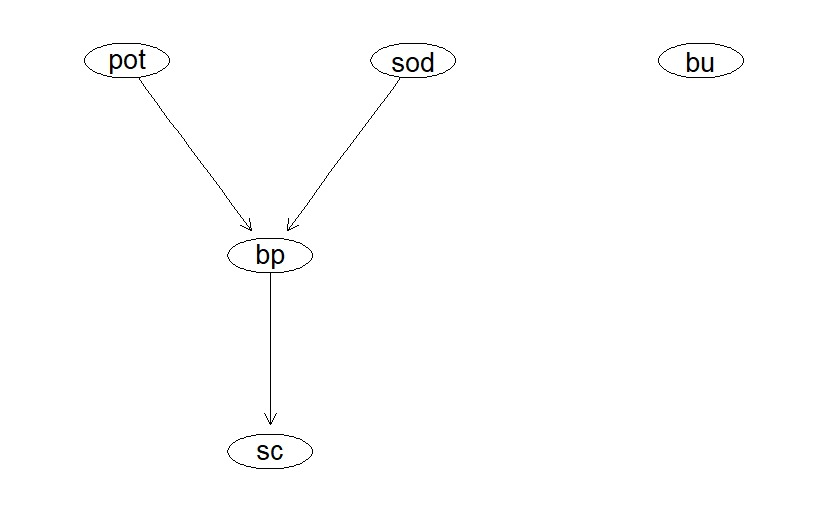
\includegraphics[width=\textwidth]{DAG1N.jpeg}
        \caption{DAG 1}
        \label{fig:dag1}
    \end{subfigure}
    \hfill
    \begin{subfigure}[b]{0.31\textwidth}
        \centering
        \includegraphics[width=\textwidth]{DAG2.1.jpeg}
        \caption{DAG 2}
        \label{fig:dag2}
    \end{subfigure}
    \hfill
    \begin{subfigure}[b]{0.31\textwidth}
        \centering
        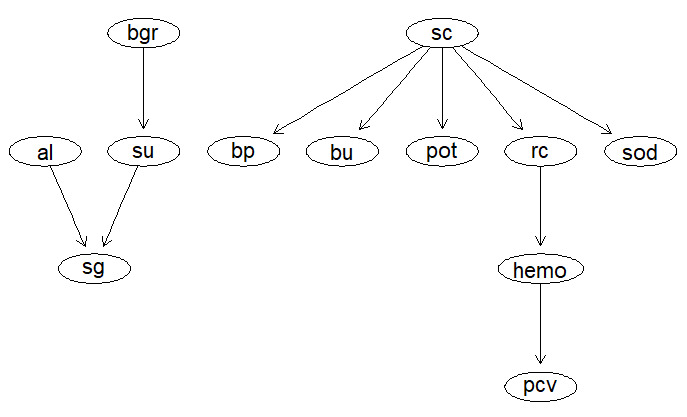
\includegraphics[width=\textwidth]{DAG3N.jpeg}
        \caption{DAG 3}
        \label{fig:dag3}
    \end{subfigure}

    \caption{DAGs propuestos para representar las relaciones 
    de dependencia entre las variables de interés.}
    \label{fig:dags}
\end{figure}


\begin{table}[htbp]
    \centering
    \caption{Comparación de los modelos lineales y no paramétricos mediante los criterios BIC y AIC.}
    \label{tab:aic_bic_dags}
    
    \resizebox{\textwidth}{!}{%
    \begin{tabular}{lrrrrlr}
        \toprule
        \textbf{DAG} &
        \textbf{BIC lineal} &
        \makecell{\textbf{BIC no}\\\textbf{paramétrico}} &
        \textbf{Mejor BIC} &
        \textbf{AIC lineal} &
        \makecell{\textbf{AIC no}\\\textbf{paramétrico}} &
        \textbf{Mejor AIC} \\
        \midrule
        
        DAG 1 &
        \textbf{-5458.132} &
        -5465.007 &
        \makecell[l]{Lineal\\(+6.875)} &
        -5434.101 &
        \textbf{-5431.521} &
        \makecell[l]{No param.\\(+2.580)} \\
        
        \addlinespace
        
        DAG 2 &
        -4810.54 &
        \textbf{-4774.671} &
        \makecell[l]{No param.\\(+35.869)} &
        -4781.244 &
        \textbf{-4720.92} &
        \makecell[l]{No param.\\(+60.324)} \\
        
        \addlinespace
        
        DAG 3 &
        -5693.505 &
        \textbf{-5605.652} &
        \makecell[l]{No param.\\(+87.853)} &
        -5636.931 &
        \textbf{-5481.793} &
        \makecell[l]{No param.\\(+155.138)} \\
        
        \bottomrule
    \end{tabular}%
    }
    
    \begin{flushleft}
        \footnotesize
        \textit{Nota.} Los valores entre paréntesis indican la diferencia 
        entre el mejor modelo y la alternativa dentro de cada DAG.
    \end{flushleft}
\end{table}

\subsubsection{Comparación entre el modelo lineal y no paramétrico}

Se evaluó si el uso de un modelo no paramétrico mejoraba los criterios de
información respecto al modelo lineal. Para BIC, el modelo lineal obtuvo un
score de $-4810.540$, mientras que el modelo no paramétrico alcanzó
$-4774.671$, lo que representa una mejora de $35.869$ unidades. De manera
similar, el AIC aumentó de $-4781.244$ en el modelo lineal a $-4720.92$ en
el modelo no paramétrico, correspondiente a una diferencia de $+60.324$
unidades. Estos resultados indican que la incorporación del
modelo no paramétrico mejora tanto el BIC como el AIC de la DAG 2. Sin embargo,
en este trabajo las consultas probabilísticas posteriores fueron realizadas
sobre el ajuste lineal de la red, por lo que el modelo no paramétrico se
utilizó únicamente como una alternativa para evaluar la calidad de ajuste.

\subsubsection{Consultas probabilísticas}
La primera consulta evaluó la probabilidad de presentar niveles elevados de
creatinina sérica, definidos como $\mathrm{sc}>1.4$, dado un nivel de sodio
superior a 145. El modelo estimó una probabilidad de $0.6277$, equivalente
al $62.77\%$.

Al agregar como evidencia simultánea un nivel de potasio mayor o igual a
5.1, la probabilidad estimada de creatinina sérica elevada fue de $0.6284$
($62.84\%$). Por lo tanto, la incorporación del potasio elevado produjo un
cambio reducido en la probabilidad estimada respecto a considerar únicamente
el sodio elevado.

En la tercera consulta se evaluó la probabilidad de presentar hiperpotasemia,
definida como un nivel de potasio mayor o igual a 5.1, en presencia de
creatinina sérica superior a 1.4 y urea superior a 40. La probabilidad
obtenida fue de $0.4313$, correspondiente al $43.13\%$.

La cuarta consulta estimó la probabilidad de presentar anemia, operacionalizada
como una concentración de hemoglobina inferior a 12 g/dL, dado un nivel de
creatinina sérica de 3.0 mg/dL y un conteo de eritrocitos de
3.5 millones/$\mu$L. La red estimó una probabilidad de $0.8096$, equivalente
al $80.96\%$.

Finalmente, para pacientes con presión arterial superior a 140, el modelo
estimó una probabilidad de $1.0000$ de presentar creatinina sérica superior
a 1.4. Este resultado corresponde a la distribución probabilística aprendida
por la red a partir de los datos utilizados y debe interpretarse dentro de
los límites del modelo.

\begin{table}[htbp]
    \centering
    \caption{Resultados de las consultas probabilísticas realizadas sobre 
    el modelo lineal de la DAG 2.}
    \label{tab:queries_dag2}
    
    \resizebox{\textwidth}{!}{%
    \begin{tabular}{cllc}
        \toprule
        \textbf{Consulta} &
        \textbf{Evento de interés} &
        \textbf{Evidencia} &
        \textbf{Probabilidad} \\
        \midrule
        
        $Q_1$ &
        $\mathrm{sc}>1.4$ &
        $\mathrm{sod}>145$ &
        $0.6277\;(62.77\%)$ \\
        
        $Q_2$ &
        $\mathrm{sc}>1.4$ &
        $\mathrm{sod}>145,\ \mathrm{pot}\geq5.1$ &
        $0.6284\;(62.84\%)$ \\
        
        $Q_3$ &
        $\mathrm{pot}\geq5.1$ &
        $\mathrm{sc}>1.4,\ \mathrm{bu}>40$ &
        $0.4313\;(43.13\%)$ \\
        
        $Q_4$ &
        $\mathrm{hemo}<12$ &
        $\mathrm{sc}=3.0,\ \mathrm{rc}=3.5$ &
        $0.8096\;(80.96\%)$ \\
        
        $Q_5$ &
        $\mathrm{sc}>1.4$ &
        $\mathrm{bp}>140$ &
        $1.0000\;(100\%)$ \\
        
        \bottomrule
    \end{tabular}%
    }
    
    \begin{flushleft}
        \footnotesize
        \textit{Nota.} 
        Las consultas $Q_1$, $Q_2$, $Q_3$ y $Q_5$ utilizaron muestreo lógico
        (\texttt{method = "ls"}), mientras que $Q_4$ utilizó ponderación por
        verosimilitud (\texttt{method = "lw"}).
    \end{flushleft}
\end{table}


\subsection{Discuciones}
\subsubsection{ajuste de la DAG2}
Los criterios de información mostraron una preferencia consistente por la
DAG 2 frente a las otras estructuras propuestas. Debido a que BIC y AIC
penalizan la complejidad del modelo además de considerar su ajuste a los
datos, el resultado sugiere que las relaciones de dependencia representadas
por esta estructura proporcionan un balance más favorable entre ajuste y
complejidad dentro de las alternativas evaluadas.

Al estudiar específicamente la DAG 2, el modelo no paramétrico obtuvo mejores
scores que el modelo lineal para ambos criterios. El incremento de $35.869$
unidades en BIC y de $60.324$ unidades en AIC indica que la alternativa no
paramétrica logró representar de mejor manera los datos de esta estructura
de acuerdo con ambos criterios. Este resultado sugiere que algunas de las
relaciones entre los biomarcadores podrían no quedar completamente descritas
por una dependencia estrictamente lineal.

\subsubsection{interpretación de las consultas}
Las consultas $Q_1$ y $Q_2$ permiten estudiar el efecto de agregar nueva
evidencia al modelo. Cuando únicamente se condicionó por sodio elevado,
la probabilidad de creatinina sérica elevada fue de $62.77\%$. Al incorporar
adicionalmente un nivel elevado de potasio, la probabilidad aumentó a
$62.84\%$, una diferencia de aproximadamente $0.07$ puntos porcentuales.

Dentro de la estructura y parametrización de la DAG 2, este cambio es
mínimo, lo cual sugiere que la evidencia adicional proporcionada por el
potasio aporta poca información para modificar la probabilidad posterior
de creatinina elevada una vez conocido el nivel alto de sodio. Sin embargo,
este resultado describe una dependencia probabilística dentro del modelo y
no implica que el potasio carezca de relevancia clínica en la enfermedad
renal.

En $Q_3$, la presencia conjunta de creatinina y urea elevadas produjo una
probabilidad estimada de hiperpotasemia del $43.13\%$. El resultado indica
que, aun bajo dicha evidencia, el modelo no asigna una probabilidad mayor
al $50\%$ al evento de hiperpotasemia. Esto muestra que la presencia de
creatinina y urea elevadas no determina de manera automática un nivel
elevado de potasio dentro de la distribución aprendida por la red.

Este comportamiento resulta relevante porque evidencia una de las ventajas
de un modelo probabilístico: la presencia de ciertos biomarcadores alterados
no conduce necesariamente a un resultado determinista en los demás nodos,
sino a una actualización de sus distribuciones condicionales.

La consulta $Q_4$ presentó una de las probabilidades más altas obtenidas.
Ante una creatinina sérica de 3.0 mg/dL y un conteo de eritrocitos de
3.5 millones/$\mu$L, la red estimó una probabilidad de $80.96\%$ de observar
una concentración de hemoglobina inferior a 12 g/dL.

Este resultado muestra cómo la combinación de evidencia proveniente de un
marcador asociado con la función renal y de un parámetro hematológico puede
modificar sustancialmente la distribución posterior de la hemoglobina.
Debe enfatizarse que esta asociación corresponde a la distribución aprendida
por la red y no demuestra por sí misma una relación causal entre las
variables.

La consulta $Q_5$ produjo una probabilidad estimada de $1.0$ para creatinina
sérica elevada cuando la presión arterial fue superior a 140. Aunque dentro
del modelo este resultado corresponde a una probabilidad del $100\%$, no
debe interpretarse como una regla clínica determinista ni generalizarse a
la población.

Un valor extremo de este tipo puede depender de la distribución aprendida
por la red, del número de observaciones disponibles en la región definida
por $\mathrm{bp}>140$, de la estructura de la DAG y del procedimiento de
inferencia aproximada. Por ello, el resultado se interpreta exclusivamente
como una propiedad del modelo ajustado a la muestra analizada.

Una consulta adicional propuesta consistió en determinar la probabilidad de
presentar ERC a partir del nivel de glucosa y de una presión arterial elevada.
Esta consulta no pudo ser evaluada mediante la GBN construida, debido a que
el evento de interés corresponde a \texttt{class}, una variable categórica
con niveles \texttt{ckd} y \texttt{notckd}.

La red utilizada en el presente estudio fue planteada como una red bayesiana
gaussiana para variables continuas, por lo que incorporar \texttt{class}
como si fuese una variable numérica continua no sería metodológicamente
apropiado. Una extensión del trabajo podría emplear una red bayesiana
gaussiana condicional, capaz de incorporar conjuntamente variables discretas
y continuas, o bien una red bayesiana completamente discreta después de
definir intervalos clínicamente justificables para los biomarcadores.

\section{Conclusiones}


%TC:ignore
%\clearpage %add new page for references
\singlespacing
\emergencystretch 3em
\hfuzz 1px
\printbibliography[heading=bibnumbered]

% \clearpage
% \begin{appendices}

% \section{Here go any appendices!}

% \end{appendices}

%TC:endignore
\end{document}